\documentclass[a4paper,twoside,10pt]{article}
\PassOptionsToPackage{utf8}{inputenc}
\PassOptionsToPackage{document}{ragged2e}
\PassOptionsToPackage{left=1.5cm,
    right=1.5cm,
    top=2.5cm,bottom=2cm}{geometry}
\parindent=0cm
\newcommand*\graysquared[1]{\tikz[baseline=(char.base)]{
    \node[fill=gray,shape=rectangle,draw,inner sep=2pt] (char) {\color{white}\textbf{#1}};}}
\newcommand*\whitesquared[1]{\tikz[baseline=(char.base)]{
    \node[fill=white,shape=rectangle,draw,inner sep=2pt] (char) {\color{black}\textbf{#1}};}}
\newcommand*\ptyxMCQcircled[1]{\tikz[baseline=(char.base)]{
    \node[shape=circle,fill=blue!20!white,draw,inner sep=2pt] (char) {\textbf{#1}};}}
\makeatletter
\newcommand{\ptyxMCQsimfill}{%
\leavevmode \cleaders \hb@xt@ .50em{\hss $\sim$\hss }\hfill \kern \z@
}
\makeatother
\newcounter{answerNumber}
\renewcommand{\thesubsection}{\Alph{subsection}}


\usepackage{inputenc}
\usepackage[T1]{fontenc}
\usepackage{ragged2e}
\usepackage{geometry}
\usepackage{pifont}
\usepackage{textcomp}
\usepackage{nopageno}
\usepackage{tikz}
\usepackage{everypage}
\usepackage{tabularx}
\usepackage{amsmath}
\usepackage{amssymb}
\usepackage{colortbl}
\usetikzlibrary{calc}
\usetikzlibrary{math}
\usepackage{zref-user}
\usepackage{zref-abspos}
\usepackage{zref-abspage}
\usepackage{zref-lastpage}

\makeatletter
\newcommand\dimtomm[1]{%
    \strip@pt\dimexpr 0.351459804\dimexpr#1\relax\relax%
}
\makeatother

\newcommand{\checkBox}[2]{%
    \begin{tikzpicture}[baseline=-12pt,color=black, thick]
        \draw[fill=#1] (0,0)
            node {\zsavepos{#2-ll}}
            rectangle (.5,-.5);
    \end{tikzpicture}%
    \write\mywrite{#2: p\thepage, (%
        \dimtomm{\zposx{#2-ll}sp},
        \dimtomm{\zposy{#2-ll}sp})%
    }%
}
\newwrite\mywrite
\openout\mywrite=\jobname.pos\relax
\AddEverypageHook{\CustomHeader}

\usepackage{enumitem} % To resume an enumeration.
\setenumerate[0]{label=\protect\ptyxMCQcircled{\arabic*}}
\newlength{\ptyxMCQTabLength}
\newcommand{\ptyxMCQTab}[2]{%
  \settowidth{\ptyxMCQTabLength}{#1{}#2}
  \ifdim \ptyxMCQTabLength<\textwidth%
  \begin{tabular}{l@{\,\,}l}#1&#2\end{tabular}%
  \else%
  \begin{tabularx}{\linewidth}{l@{\,\,}X}#1&#2\end{tabularx}%
  \fi%
}



\begin{document}
\newcommand\CustomHeader{%
    \begin{tikzpicture}[remember picture,overlay,black,every node/.style={inner sep=0,outer sep=-0.2}]
        \draw[fill=black] ([xshift=1cm,yshift=-1cm]current page.north west)
            rectangle ([xshift=1.5cm,yshift=-1.5cm]current page.north west);
        \draw[fill=black] ([xshift=-1cm,yshift=-1cm]current page.north east)
            rectangle ([xshift=-1.5cm,yshift=-1.5cm]current page.north east);
        \draw[fill=black] ([xshift=1cm,yshift=1cm]current page.south west)
            rectangle ([xshift=1.5cm,yshift=1.5cm]current page.south west);
        \draw[fill=black] ([xshift=-1cm,yshift=1cm]current page.south east)
            rectangle ([xshift=-1.5cm,yshift=1.5cm]current page.south east);\node at ([yshift=-1cm]current page.north) [anchor=north] {
            \begin{tikzpicture}
            \definecolor{color0}{rgb}{1,1,1}
            \definecolor{color1}{rgb}{0,0,0}
            \draw[fill=black] (0,0) rectangle (0.25,0.25);
            \tikzmath {
    \n=\thepage;
    \j=0;
    for \i in {1,...,8}{%
            \r = int(Mod(\n,2));
            \n = int(\n/2);
            {\draw[fill=color\r] ({\i*0.25+2*\j},0) rectangle ({\i*0.25+0.25+2*\j},0.25);
             };
            };
    \n=1;
    \j=1;
    for \i in {1,...,8}{%
            \r = int(Mod(\n,2));
            \n = int(\n/2);
            {\draw[fill=color\r] ({\i*0.25+2*\j},0) rectangle ({\i*0.25+0.25+2*\j},0.25);
             };
            };
    \n=0;
    \j=2;
    for \i in {1,...,8}{%
            \r = int(Mod(\n,2));
            \n = int(\n/2);
            {\draw[fill=color\r] ({\i*0.25+2*\j},0) rectangle ({\i*0.25+0.25+2*\j},0.25);
             };
            };}
        \node[anchor=west] at  ({2.5+2*\j},0.1)
            {\scriptsize\textbf{\#1}~:~{\thepage}/\zpageref{LastPage}};
        \end{tikzpicture}};

        \draw[dotted]  ([xshift=-1cm,yshift=-2cm]current page.north east)
            -- ([xshift=1cm,yshift=-2cm]current page.north west)
            node [pos=0.25,fill=white]
            {\,\,\scriptsize\textuparrow\,\,\textsc{N'écrivez rien au
            dessus de cette ligne}\,\,\textuparrow\,\,}
            node [pos=0.75,fill=white]
            {\,\,\scriptsize\textuparrow\,\,\textsc{N'écrivez rien au
            dessus de cette ligne}\,\,\textuparrow\,\,};
    \end{tikzpicture}}



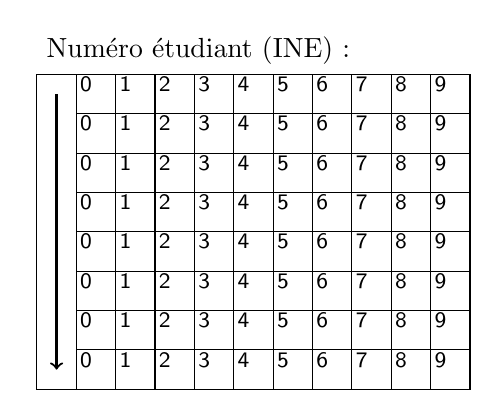
\begin{tikzpicture}[baseline=-10pt,scale=.5]
\node[anchor=south west] at (-1, 0) {Numéro étudiant (INE)~:};
\draw[] (-1, 0) node {\zsavepos{ID-table}} rectangle (0,-8);
\draw (0,0) rectangle (1,-1)
                    (0.25,-0.25) node  {\footnotesize\color{black}\textsf{0}};
\draw (1,0) rectangle (2,-1)
                    (1.25,-0.25) node  {\footnotesize\color{black}\textsf{1}};
\draw (2,0) rectangle (3,-1)
                    (2.25,-0.25) node  {\footnotesize\color{black}\textsf{2}};
\draw (3,0) rectangle (4,-1)
                    (3.25,-0.25) node  {\footnotesize\color{black}\textsf{3}};
\draw (4,0) rectangle (5,-1)
                    (4.25,-0.25) node  {\footnotesize\color{black}\textsf{4}};
\draw (5,0) rectangle (6,-1)
                    (5.25,-0.25) node  {\footnotesize\color{black}\textsf{5}};
\draw (6,0) rectangle (7,-1)
                    (6.25,-0.25) node  {\footnotesize\color{black}\textsf{6}};
\draw (7,0) rectangle (8,-1)
                    (7.25,-0.25) node  {\footnotesize\color{black}\textsf{7}};
\draw (8,0) rectangle (9,-1)
                    (8.25,-0.25) node  {\footnotesize\color{black}\textsf{8}};
\draw (9,0) rectangle (10,-1)
                    (9.25,-0.25) node  {\footnotesize\color{black}\textsf{9}};
\draw (9,0) rectangle (10,-1);
\draw (0,-1) rectangle (1,-2)
                    (0.25,-1.25) node  {\footnotesize\color{black}\textsf{0}};
\draw (1,-1) rectangle (2,-2)
                    (1.25,-1.25) node  {\footnotesize\color{black}\textsf{1}};
\draw (2,-1) rectangle (3,-2)
                    (2.25,-1.25) node  {\footnotesize\color{black}\textsf{2}};
\draw (3,-1) rectangle (4,-2)
                    (3.25,-1.25) node  {\footnotesize\color{black}\textsf{3}};
\draw (4,-1) rectangle (5,-2)
                    (4.25,-1.25) node  {\footnotesize\color{black}\textsf{4}};
\draw (5,-1) rectangle (6,-2)
                    (5.25,-1.25) node  {\footnotesize\color{black}\textsf{5}};
\draw (6,-1) rectangle (7,-2)
                    (6.25,-1.25) node  {\footnotesize\color{black}\textsf{6}};
\draw (7,-1) rectangle (8,-2)
                    (7.25,-1.25) node  {\footnotesize\color{black}\textsf{7}};
\draw (8,-1) rectangle (9,-2)
                    (8.25,-1.25) node  {\footnotesize\color{black}\textsf{8}};
\draw (9,-1) rectangle (10,-2)
                    (9.25,-1.25) node  {\footnotesize\color{black}\textsf{9}};
\draw (9,-1) rectangle (10,-2);
\draw (0,-2) rectangle (1,-3)
                    (0.25,-2.25) node  {\footnotesize\color{black}\textsf{0}};
\draw (1,-2) rectangle (2,-3)
                    (1.25,-2.25) node  {\footnotesize\color{black}\textsf{1}};
\draw (2,-2) rectangle (3,-3)
                    (2.25,-2.25) node  {\footnotesize\color{black}\textsf{2}};
\draw (3,-2) rectangle (4,-3)
                    (3.25,-2.25) node  {\footnotesize\color{black}\textsf{3}};
\draw (4,-2) rectangle (5,-3)
                    (4.25,-2.25) node  {\footnotesize\color{black}\textsf{4}};
\draw (5,-2) rectangle (6,-3)
                    (5.25,-2.25) node  {\footnotesize\color{black}\textsf{5}};
\draw (6,-2) rectangle (7,-3)
                    (6.25,-2.25) node  {\footnotesize\color{black}\textsf{6}};
\draw (7,-2) rectangle (8,-3)
                    (7.25,-2.25) node  {\footnotesize\color{black}\textsf{7}};
\draw (8,-2) rectangle (9,-3)
                    (8.25,-2.25) node  {\footnotesize\color{black}\textsf{8}};
\draw (9,-2) rectangle (10,-3)
                    (9.25,-2.25) node  {\footnotesize\color{black}\textsf{9}};
\draw (9,-2) rectangle (10,-3);
\draw (0,-3) rectangle (1,-4)
                    (0.25,-3.25) node  {\footnotesize\color{black}\textsf{0}};
\draw (1,-3) rectangle (2,-4)
                    (1.25,-3.25) node  {\footnotesize\color{black}\textsf{1}};
\draw (2,-3) rectangle (3,-4)
                    (2.25,-3.25) node  {\footnotesize\color{black}\textsf{2}};
\draw (3,-3) rectangle (4,-4)
                    (3.25,-3.25) node  {\footnotesize\color{black}\textsf{3}};
\draw (4,-3) rectangle (5,-4)
                    (4.25,-3.25) node  {\footnotesize\color{black}\textsf{4}};
\draw (5,-3) rectangle (6,-4)
                    (5.25,-3.25) node  {\footnotesize\color{black}\textsf{5}};
\draw (6,-3) rectangle (7,-4)
                    (6.25,-3.25) node  {\footnotesize\color{black}\textsf{6}};
\draw (7,-3) rectangle (8,-4)
                    (7.25,-3.25) node  {\footnotesize\color{black}\textsf{7}};
\draw (8,-3) rectangle (9,-4)
                    (8.25,-3.25) node  {\footnotesize\color{black}\textsf{8}};
\draw (9,-3) rectangle (10,-4)
                    (9.25,-3.25) node  {\footnotesize\color{black}\textsf{9}};
\draw (9,-3) rectangle (10,-4);
\draw (0,-4) rectangle (1,-5)
                    (0.25,-4.25) node  {\footnotesize\color{black}\textsf{0}};
\draw (1,-4) rectangle (2,-5)
                    (1.25,-4.25) node  {\footnotesize\color{black}\textsf{1}};
\draw (2,-4) rectangle (3,-5)
                    (2.25,-4.25) node  {\footnotesize\color{black}\textsf{2}};
\draw (3,-4) rectangle (4,-5)
                    (3.25,-4.25) node  {\footnotesize\color{black}\textsf{3}};
\draw (4,-4) rectangle (5,-5)
                    (4.25,-4.25) node  {\footnotesize\color{black}\textsf{4}};
\draw (5,-4) rectangle (6,-5)
                    (5.25,-4.25) node  {\footnotesize\color{black}\textsf{5}};
\draw (6,-4) rectangle (7,-5)
                    (6.25,-4.25) node  {\footnotesize\color{black}\textsf{6}};
\draw (7,-4) rectangle (8,-5)
                    (7.25,-4.25) node  {\footnotesize\color{black}\textsf{7}};
\draw (8,-4) rectangle (9,-5)
                    (8.25,-4.25) node  {\footnotesize\color{black}\textsf{8}};
\draw (9,-4) rectangle (10,-5)
                    (9.25,-4.25) node  {\footnotesize\color{black}\textsf{9}};
\draw (9,-4) rectangle (10,-5);
\draw (0,-5) rectangle (1,-6)
                    (0.25,-5.25) node  {\footnotesize\color{black}\textsf{0}};
\draw (1,-5) rectangle (2,-6)
                    (1.25,-5.25) node  {\footnotesize\color{black}\textsf{1}};
\draw (2,-5) rectangle (3,-6)
                    (2.25,-5.25) node  {\footnotesize\color{black}\textsf{2}};
\draw (3,-5) rectangle (4,-6)
                    (3.25,-5.25) node  {\footnotesize\color{black}\textsf{3}};
\draw (4,-5) rectangle (5,-6)
                    (4.25,-5.25) node  {\footnotesize\color{black}\textsf{4}};
\draw (5,-5) rectangle (6,-6)
                    (5.25,-5.25) node  {\footnotesize\color{black}\textsf{5}};
\draw (6,-5) rectangle (7,-6)
                    (6.25,-5.25) node  {\footnotesize\color{black}\textsf{6}};
\draw (7,-5) rectangle (8,-6)
                    (7.25,-5.25) node  {\footnotesize\color{black}\textsf{7}};
\draw (8,-5) rectangle (9,-6)
                    (8.25,-5.25) node  {\footnotesize\color{black}\textsf{8}};
\draw (9,-5) rectangle (10,-6)
                    (9.25,-5.25) node  {\footnotesize\color{black}\textsf{9}};
\draw (9,-5) rectangle (10,-6);
\draw (0,-6) rectangle (1,-7)
                    (0.25,-6.25) node  {\footnotesize\color{black}\textsf{0}};
\draw (1,-6) rectangle (2,-7)
                    (1.25,-6.25) node  {\footnotesize\color{black}\textsf{1}};
\draw (2,-6) rectangle (3,-7)
                    (2.25,-6.25) node  {\footnotesize\color{black}\textsf{2}};
\draw (3,-6) rectangle (4,-7)
                    (3.25,-6.25) node  {\footnotesize\color{black}\textsf{3}};
\draw (4,-6) rectangle (5,-7)
                    (4.25,-6.25) node  {\footnotesize\color{black}\textsf{4}};
\draw (5,-6) rectangle (6,-7)
                    (5.25,-6.25) node  {\footnotesize\color{black}\textsf{5}};
\draw (6,-6) rectangle (7,-7)
                    (6.25,-6.25) node  {\footnotesize\color{black}\textsf{6}};
\draw (7,-6) rectangle (8,-7)
                    (7.25,-6.25) node  {\footnotesize\color{black}\textsf{7}};
\draw (8,-6) rectangle (9,-7)
                    (8.25,-6.25) node  {\footnotesize\color{black}\textsf{8}};
\draw (9,-6) rectangle (10,-7)
                    (9.25,-6.25) node  {\footnotesize\color{black}\textsf{9}};
\draw (9,-6) rectangle (10,-7);
\draw (0,-7) rectangle (1,-8)
                    (0.25,-7.25) node  {\footnotesize\color{black}\textsf{0}};
\draw (1,-7) rectangle (2,-8)
                    (1.25,-7.25) node  {\footnotesize\color{black}\textsf{1}};
\draw (2,-7) rectangle (3,-8)
                    (2.25,-7.25) node  {\footnotesize\color{black}\textsf{2}};
\draw (3,-7) rectangle (4,-8)
                    (3.25,-7.25) node  {\footnotesize\color{black}\textsf{3}};
\draw (4,-7) rectangle (5,-8)
                    (4.25,-7.25) node  {\footnotesize\color{black}\textsf{4}};
\draw (5,-7) rectangle (6,-8)
                    (5.25,-7.25) node  {\footnotesize\color{black}\textsf{5}};
\draw (6,-7) rectangle (7,-8)
                    (6.25,-7.25) node  {\footnotesize\color{black}\textsf{6}};
\draw (7,-7) rectangle (8,-8)
                    (7.25,-7.25) node  {\footnotesize\color{black}\textsf{7}};
\draw (8,-7) rectangle (9,-8)
                    (8.25,-7.25) node  {\footnotesize\color{black}\textsf{8}};
\draw (9,-7) rectangle (10,-8)
                    (9.25,-7.25) node  {\footnotesize\color{black}\textsf{9}};
\draw (9,-7) rectangle (10,-8);
\draw[black,->,thick] (-0.5, -0.5) -- (-0.5,-7.5);
\end{tikzpicture}
\hfill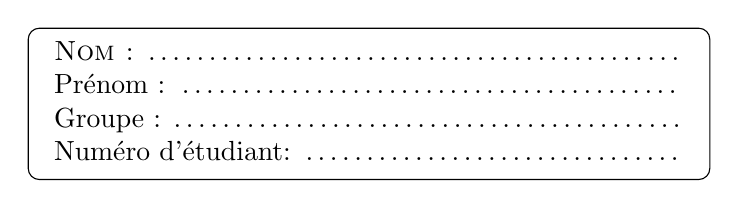
\begin{tikzpicture}[baseline=10pt]\node[draw,rounded corners] {\begin{tabular}{p{8cm}}\textsc{Nom~:}~\dotfill\\Prénom~:~\dotfill\\Groupe~:~\dotfill\\Numéro d'étudiant:~\dotfill\\\end{tabular}};\end{tikzpicture}\write\mywrite{ID-table: (\dimtomm{\zposx{ID-table}sp}, \dimtomm{\zposy{ID-table}sp})}



            \vspace{1em}

            \tikz{\draw[dotted] ([xshift=2cm]current page.west) -- ([xshift=-1cm]current page.east);}
             % (introduction)






 % (introduction)
\begin{enumerate}[resume]\pagebreak[3]\item\filbreak\setcounter{answerNumber}{0}




Let $B=\begin{pmatrix}1 & 0 & 0\\- \frac{3}{4} & 1 & 0\\\frac{83}{14} & - \frac{32}{7} & 0\end{pmatrix}$.


\nopagebreak[4]

\begin{minipage}{\textwidth}
\begin{flushleft}

\begin{minipage}{\textwidth}
\ptyxMCQTab{\checkBox{white}{Q1-1}}{answer 1}\quad
\ptyxMCQTab{\checkBox{white}{Q1-2}}{answer 2}\quad
\ptyxMCQTab{\checkBox{white}{Q1-3}}{answer 3}\quad


\end{minipage}
\end{flushleft}
\end{minipage}\pagebreak[3]\item\filbreak\setcounter{answerNumber}{0}



Question:


\nopagebreak[4]

\begin{minipage}{\textwidth}
\begin{flushleft}\ptyxMCQTab{\checkBox{white}{Q3-1}}{1}\quad
\ptyxMCQTab{\checkBox{white}{Q3-2}}{$- \frac{7}{8}$}\quad

\end{flushleft}
\end{minipage}\pagebreak[3]\item\filbreak\setcounter{answerNumber}{0}



Question:
\texttt{...................}

\nopagebreak[4]

\begin{minipage}{\textwidth}
\begin{flushleft}
\ptyxMCQTab{\checkBox{white}{Q2-2}}{\texttt{M[i0] += -M[i][j0]}}\quad
\ptyxMCQTab{\checkBox{white}{Q2-1}}{\texttt{M[i] += -M[i][j0]}}\quad

\end{flushleft}
\end{minipage}\end{enumerate}
 


\cleardoublepage
\end{document}